\chapter{Laser System Overview}
%the sum of the whole is greater than the parts 

This chapter provide a broad introduction to the laser system addressed in this thesis. More information on the Master Laser configuration and setup can be found in Chapter \ref{generationOfSeedLight}. Information about the AOM configuration can be found in Chapter \ref{AOMInstallChapter}. The process of injection locking the slave lasers is discussed in more detail in Chapter \ref{InjectionLockingChapter}. Data from the working system can be found in Chapter \ref{triumphantDataChapter}.

The purpose of this system is to produce two lasers which are near resonant with the 5s $^2$S$_{1/2}$ to 5p$^2$P$_{3/2}$ transition in $^{87}$Sr$+$, but which differ in frequency by precisely 5 GHz, which corresponds to the hyperfine splitting of the ground state. This is necessary to make the stimulated Raman transitions for our experiment. As we will later see, the experiment is less sensitive to common mode drift between the two slave lasers than it is to the drifting of individual slaves.

since, as we will find in Chapter\,\ref{ChapterAboutTheAtoms}, our ability to drive the transitions depends strongly on the difference between the lasing frequencies of our two lasers. In contrast, we expect our experiment to be relatively less sensitive to common mode drifts in the frequencies of our lasers.
The laser system consists of several components arranged together on a 12''$\times$48'' breadboard that is mounted to an optical table. The breadboard is enclosed by a plastic case. The current driver circuits and temperature controllers for the lasers are mounted on a shelf above the laser enclosure along with the RF generator, RF amplifier along with various pieces of test and measurement equipment.  A picture of the completed setup can be found in Figure\,\ref{fullexperimentphoto}. 

\begin{figure}
    \centerline{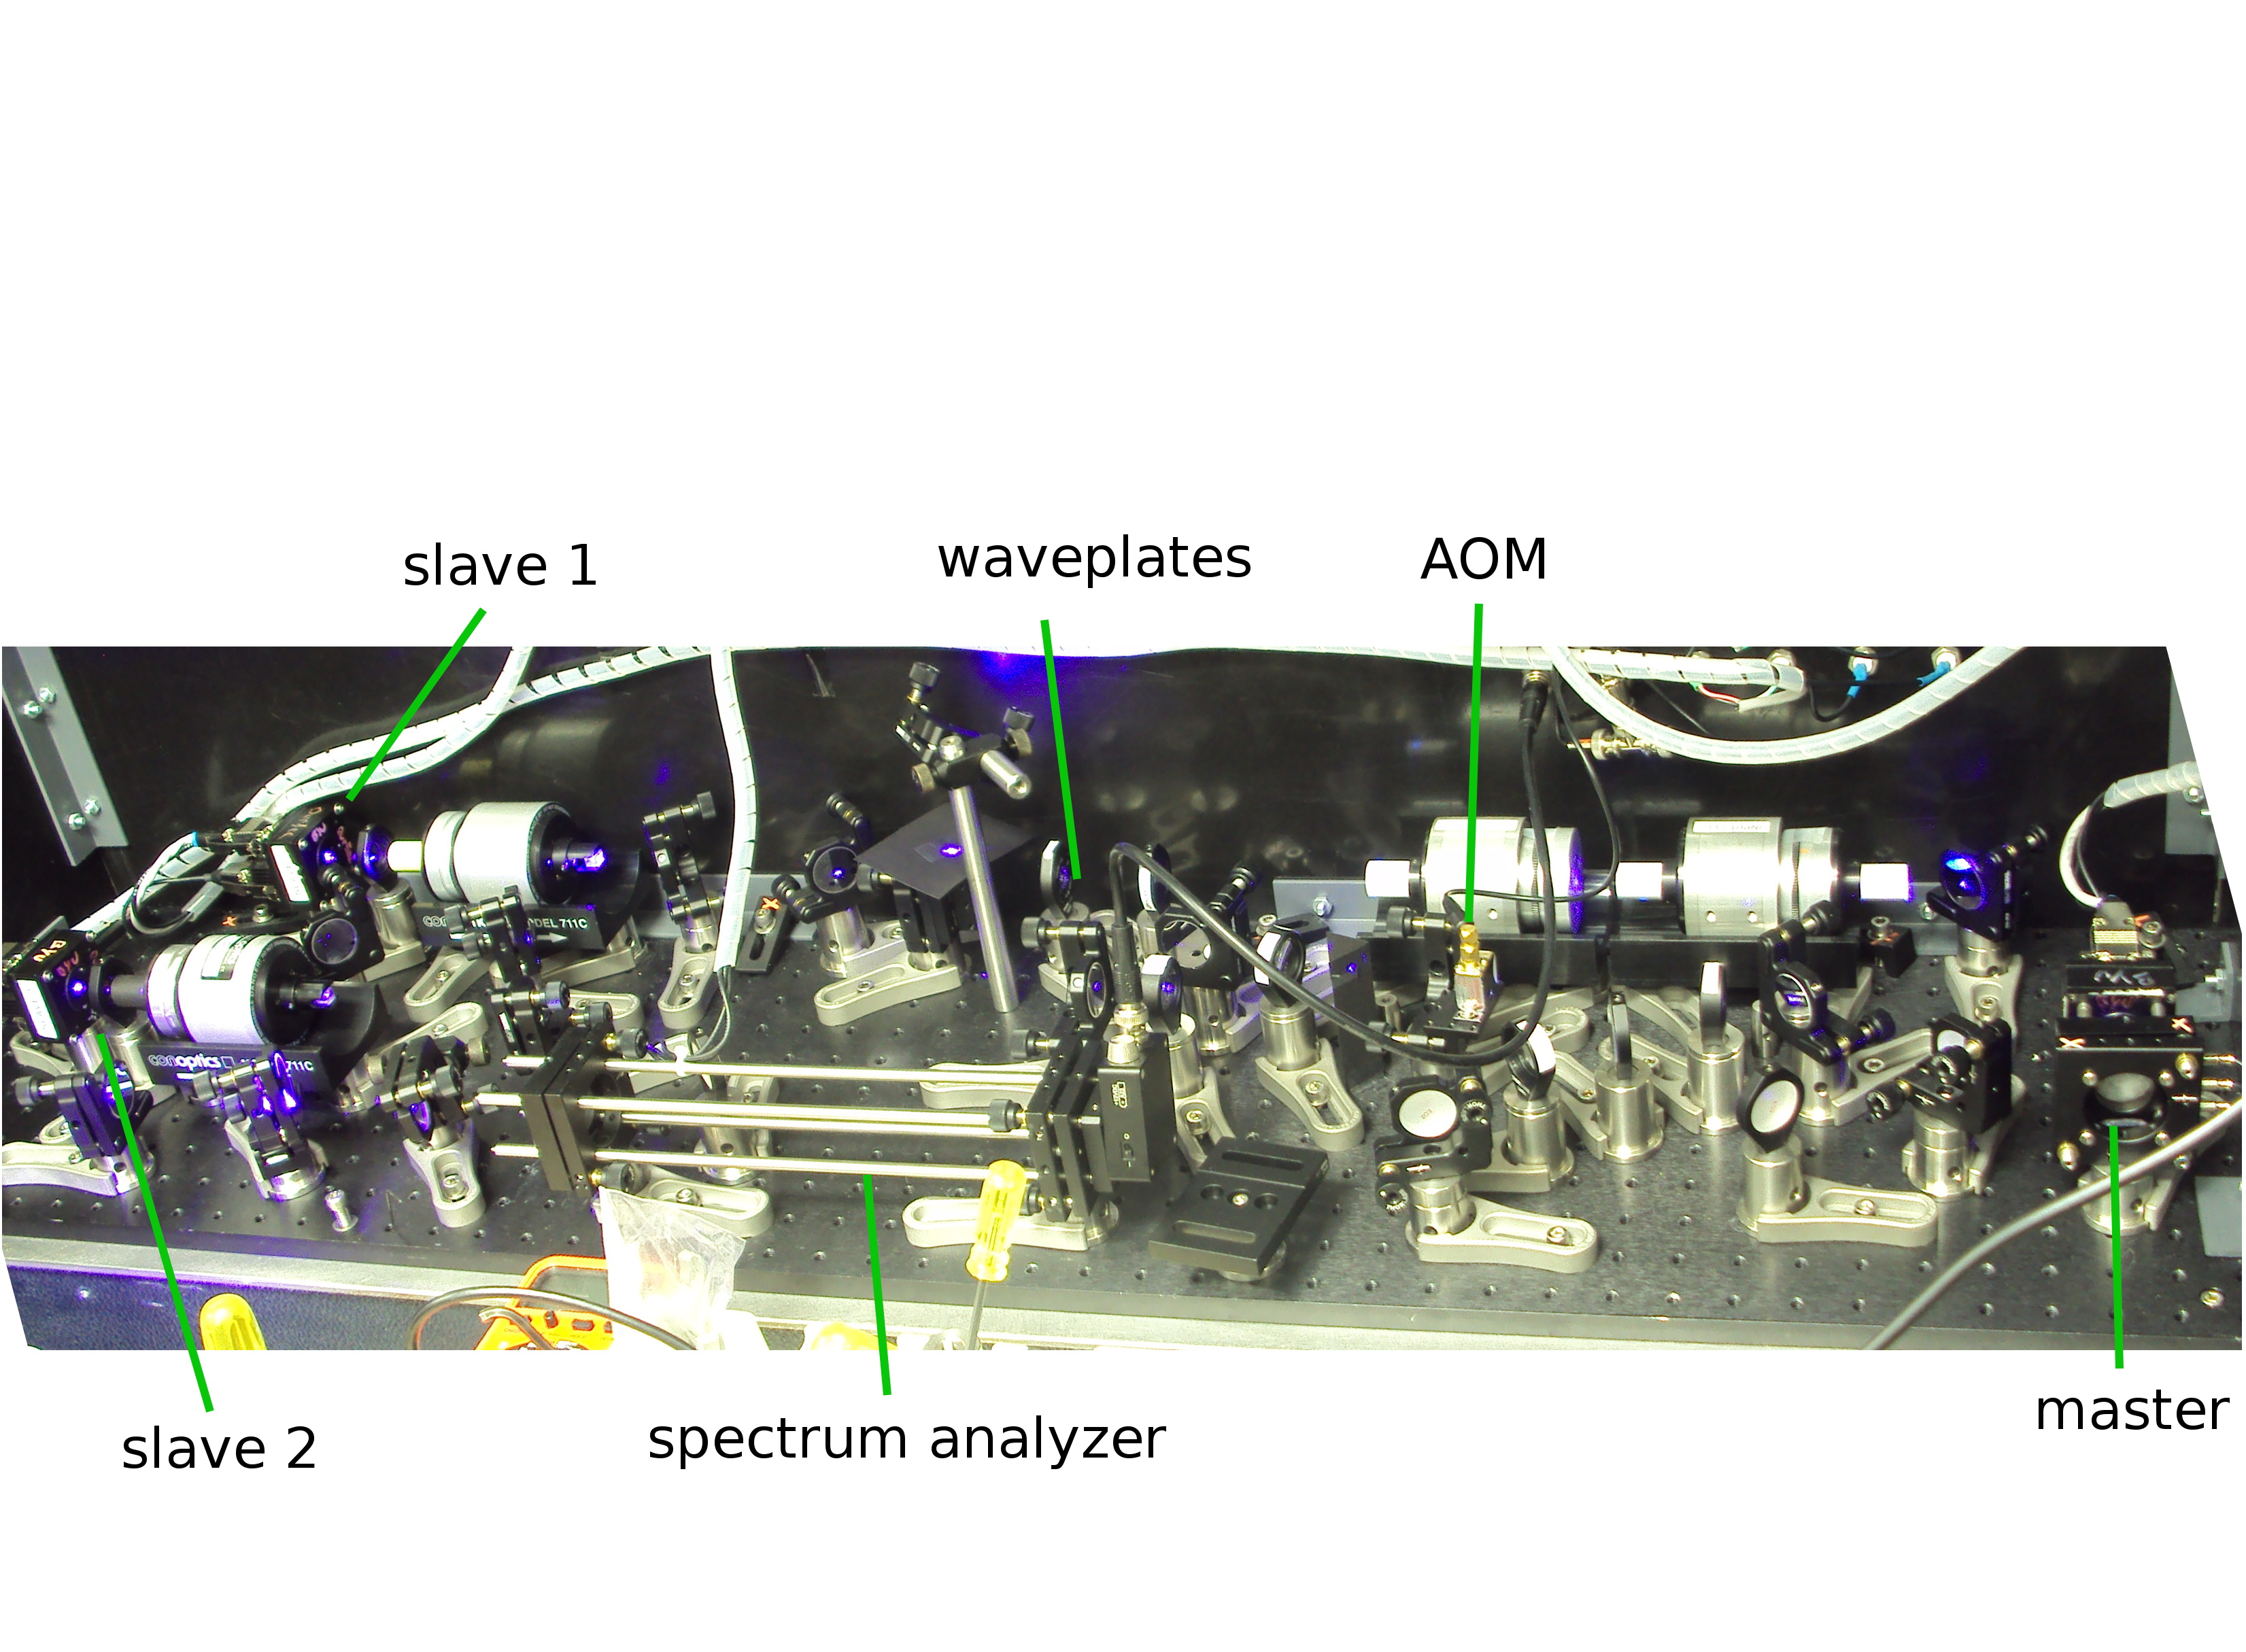
\includegraphics[width=1\textwidth]{entire_setup}}
    \caption[Photo of Entire System]{\label{fullexperimentphoto}
A photograph of the entire laser system while in operation. 
    }
\end{figure}

There are three separate laser diodes in housings. One of them is designated the ``Master'' laser. The other two are designated ``Slave 1'' and ``Slave 2.'' 
 A diagram of the main components of the system can be found in Figure\,\ref{diagramOfSetup3}.

The advantage of this setup is that if the master laser were to drift, both slaves would drift with it. The light that will actually be used on the atoms in the experiment comes out of the two slaves. The master laser is supposed to serve as a stable frequency reference so that the slave lasers can be seeded by it. Thus, the basic objective is to make a stable master laser tuned near the mean of the frequencies that we desire out of the slave lasers. This will then be shifted by an AOM and coupled into the slave lasers. The slave lasers are adjusted so that they are able to amplify the light from the AOM and lase with the same frequency as the light that comes out at the AOM. This is what is meant by ``injection locking.''

\begin{figure}
    \centerline{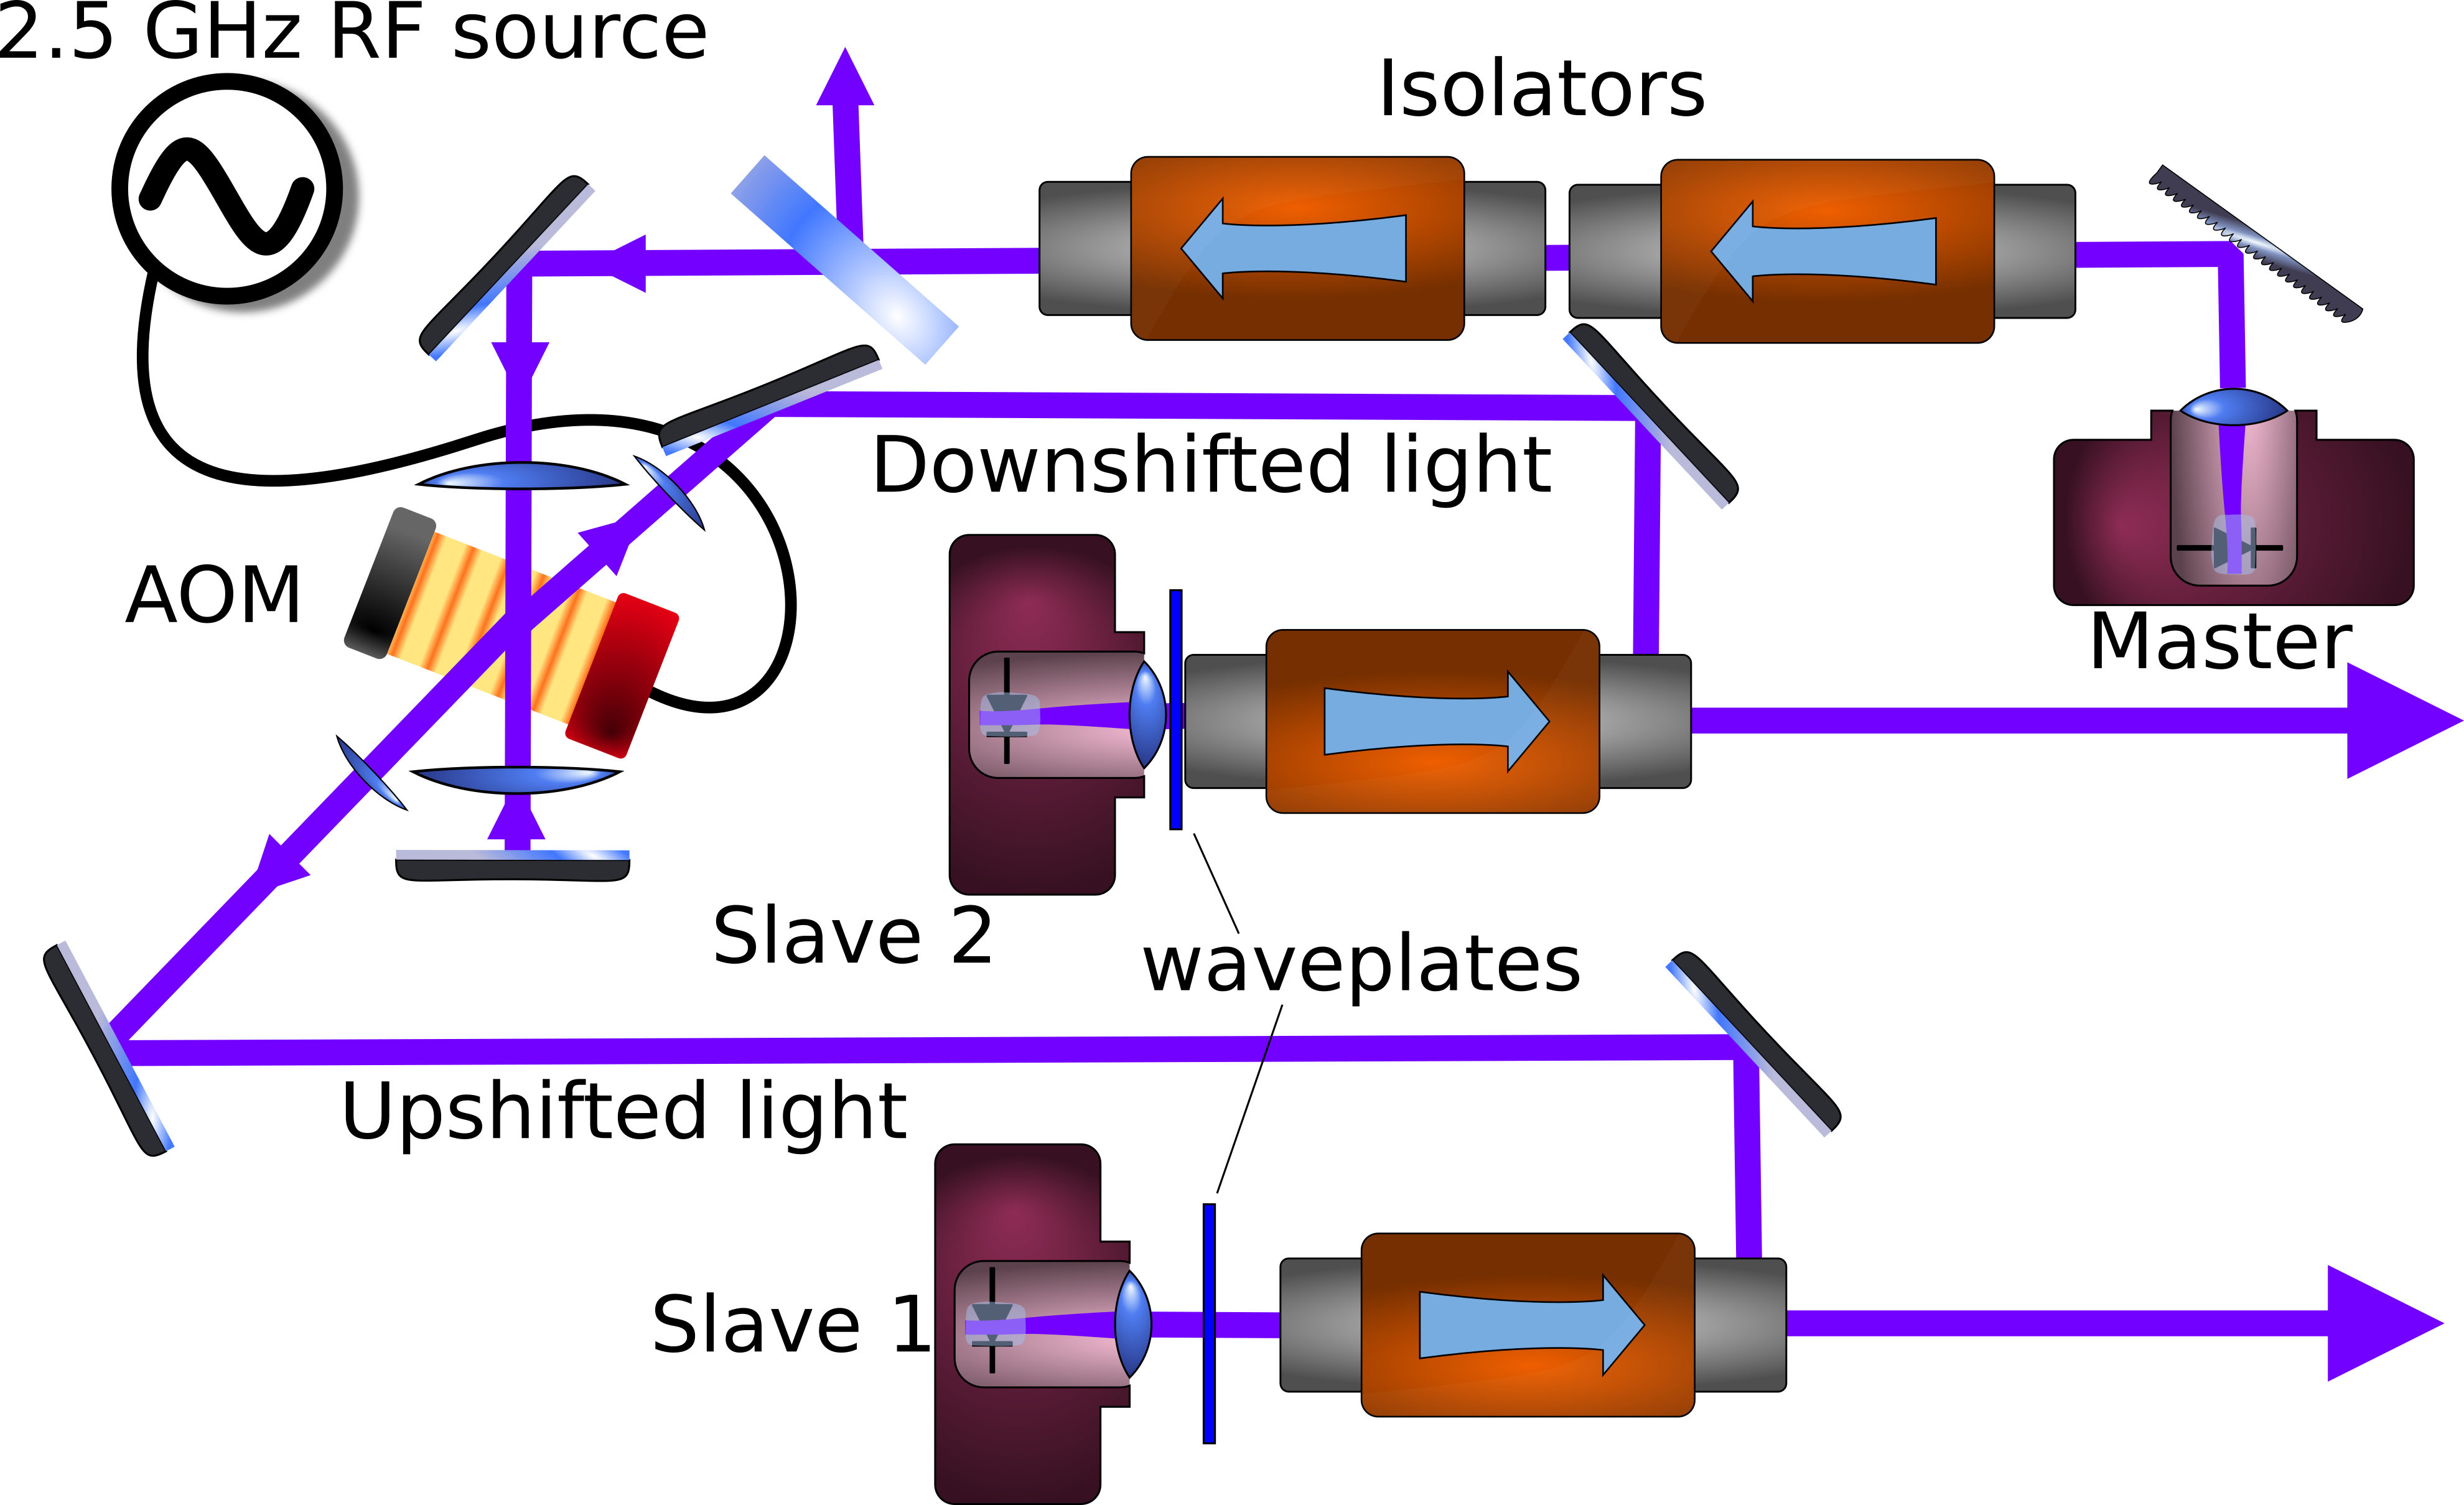
\includegraphics[width=1\textwidth]{diagramOfSetup3}}
    \caption[Diagram of the Setup]{\label{figdiagramOfSetup}
	A cartoon diagram of the basic pieces of the apparatus. The master laser is depicted on the upper right. Its beam passes through two optical isolators in series. After this, the AOM is depicted with the two beams coming out at exaggerated angles. These are then coupled into the rejection ports of two other optical isolators. Finally, the final two beams come out the other end. Not pictured is the two waveplate setup that comes near the beam splitter. Also possibly not pictured are some half waveplates that go near the slave laser.\footnote{Bad news, AOM might be in backwards} 
    }
\end{figure}

Light from the master laser passes through two optical isolators. These use Faraday rotation and a pair of glan polarizers to ensure that light travelling away from the master laser is allowed to propagate while light is prevented from coming back into the master laser. See Fig.~\ref{isolatorPicture}.

\begin{figure}
\label{isolatorPicture}
\centerline{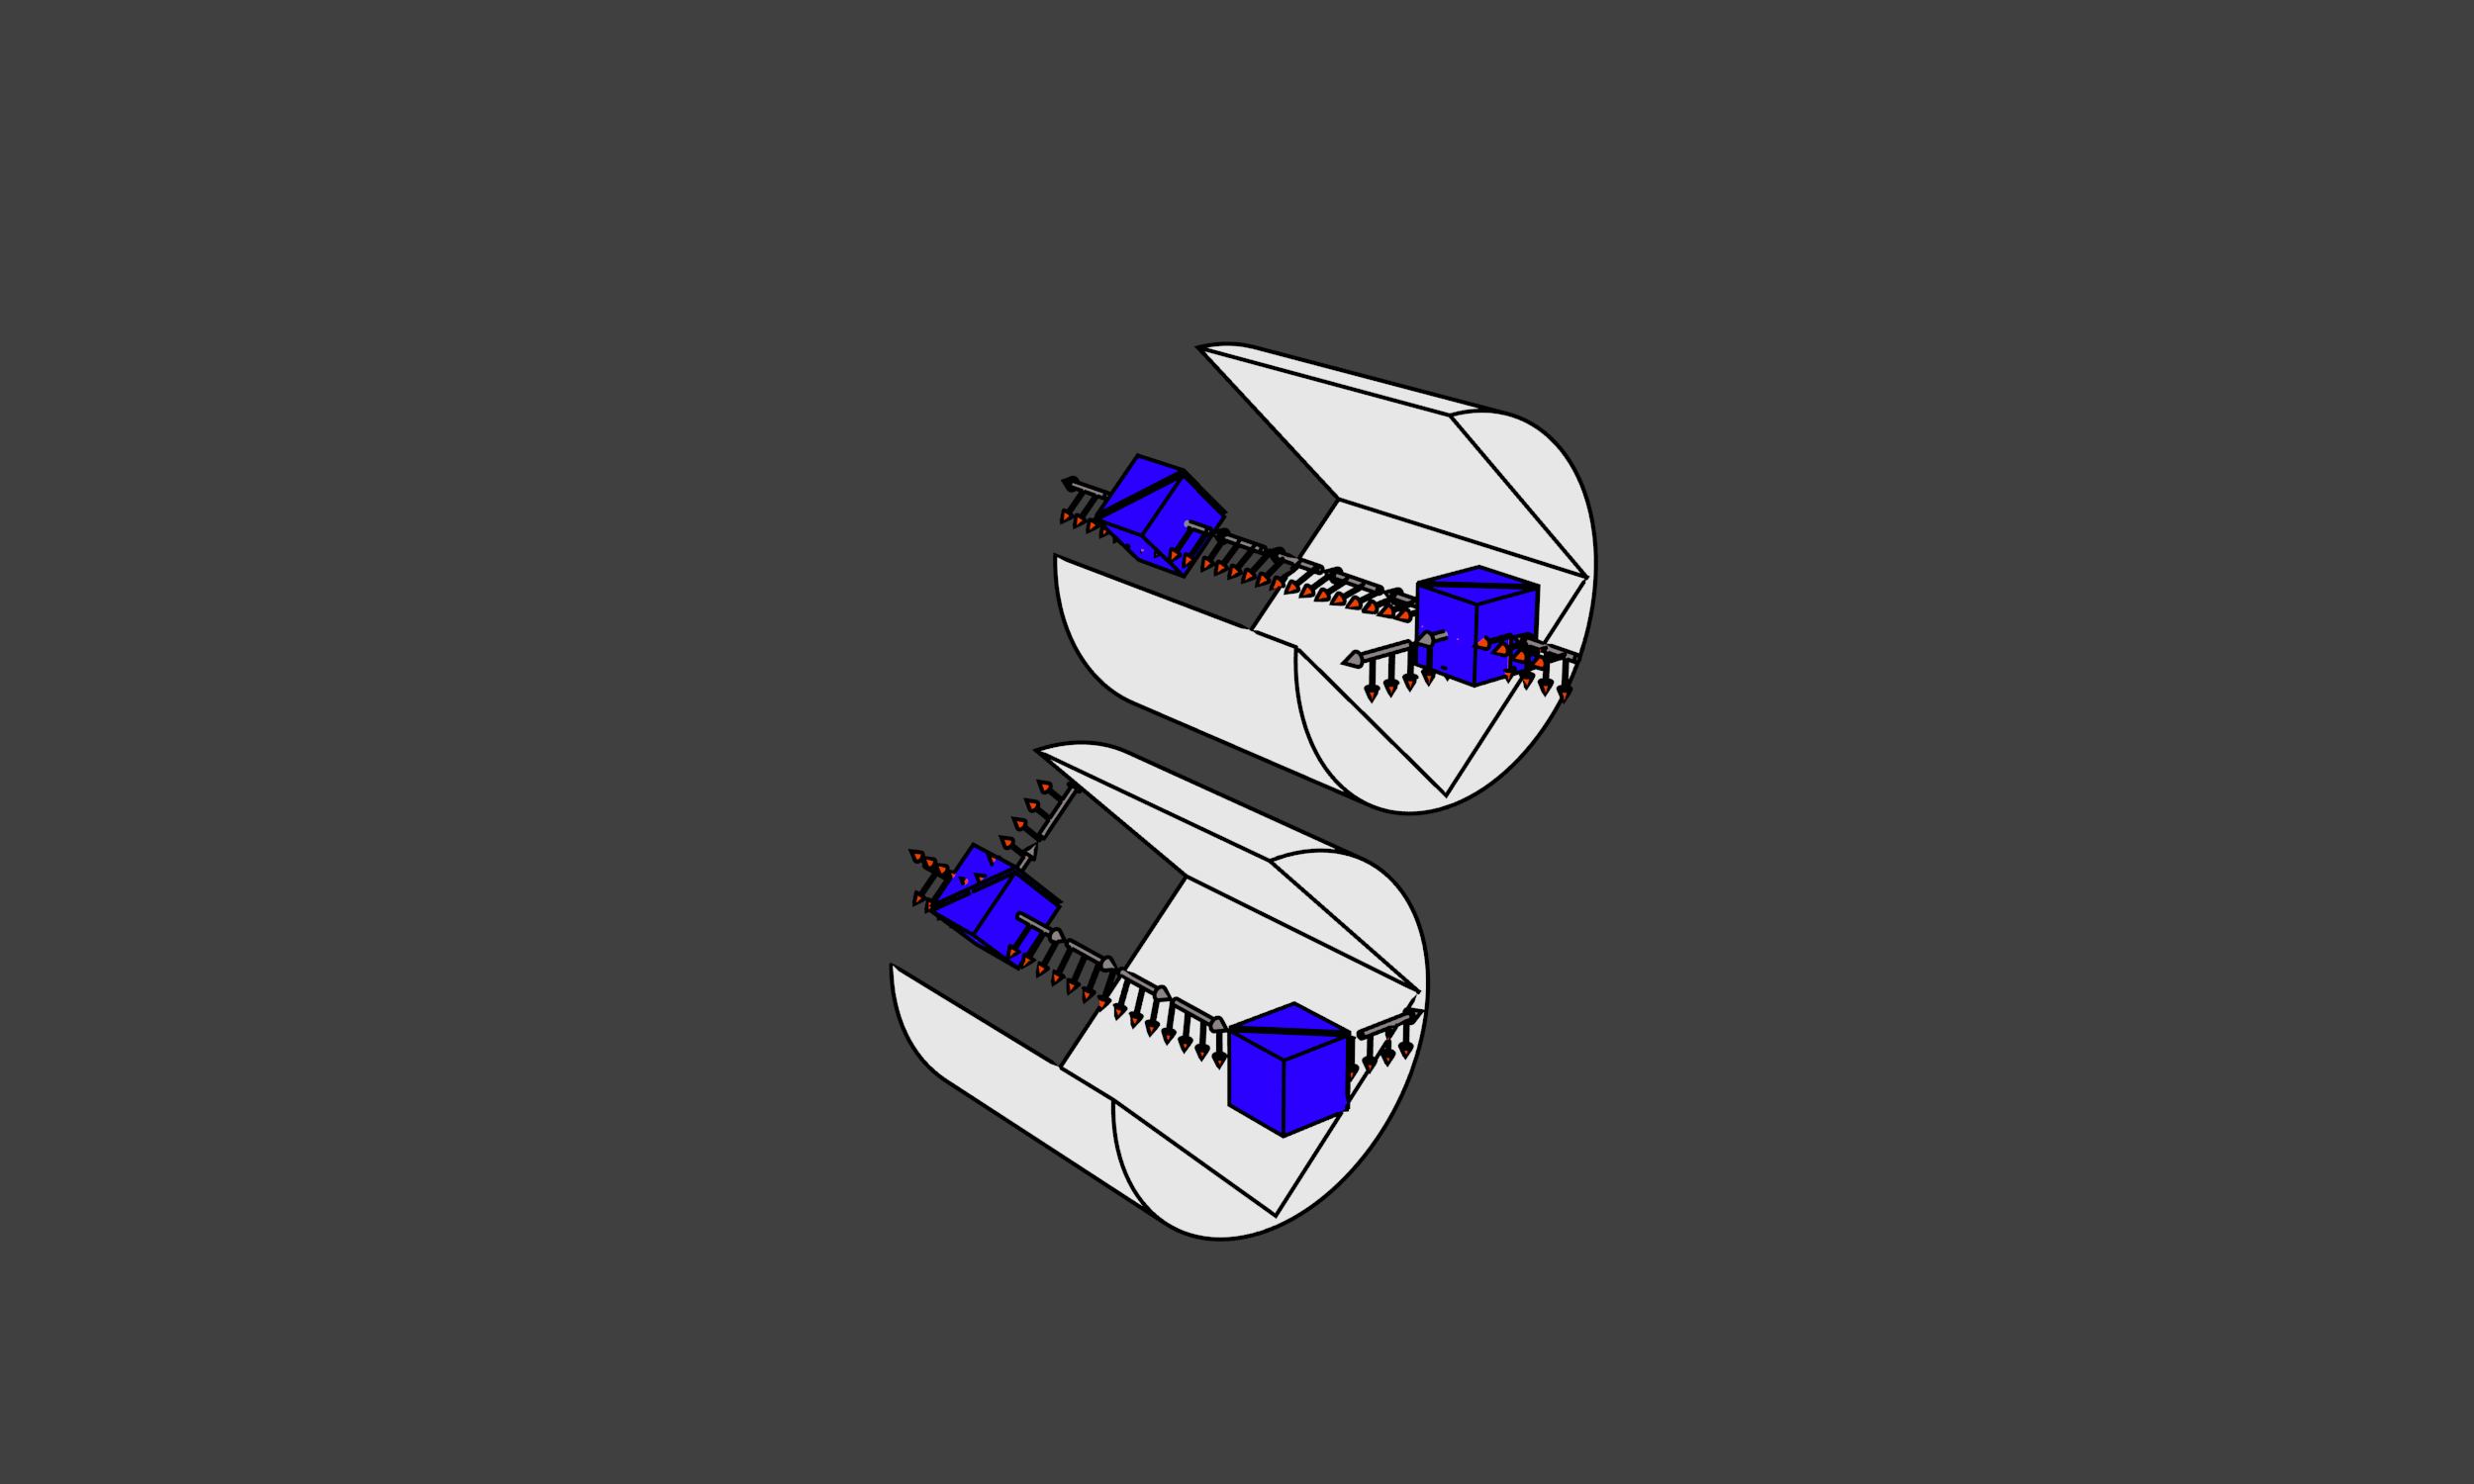
\includegraphics[width=1\textwidth]{isolators}}
\caption[Optical Isolator Illustration]{Optical isolator illustration. The gray arrows represent the direction of propagation of the light. The red arrows represent the direction of polarization.}
\end{figure}

Optical isolators are important because the stability of the master laser and the injection locking of the slave lasers requires control of the light being coupled into the laser cavity. By installing isolators, we can prevent unwanted reflections back into the master laser. This is an especially serious issue for the master laser since later in the beam path, we retroreflect the beam in such a way that, absent the isolators, light would couple directly back into the master laser. 

The beam then passes through a pair of waveplates and a polarizing beam cube, which serves the dual purpose of allowing us to attenuate the portion of the beam that goes through the AOM and splitting off a beam that can be used in our spectrum analyzer. A discussion of 

After this, the laser is passed twice through an Acousto-optic Modulator (AOM). The first-order diffracted beam from the first pass through the AOM produces light that is shifted up in frequency (down in wavelength). However, most of the power is contained in the 0th order beam that passes through the AOM without being shifted at all. We collimate this beam and retroreflect it and send it in the other direction. This pass produces a weak beam that is downshifted in frequency. We thus end up with two beams, one of which is shifted upwards by 2.5 GHz and the other of which is shifted downward by 2.5 GHz. These two beams are then coupled through optical isolators into the two slave lasers. The outputs of these two lasers are what we use in our experiment to achieve stimulated Raman transitions. 

%We could have maybe used light coming out the rejection ports to monitor second order effects from the AOM. 

Both slaves are also redirected to the spectrum analyzer. 

\section{Basic Design}
\begin{figure}
%    \centerline{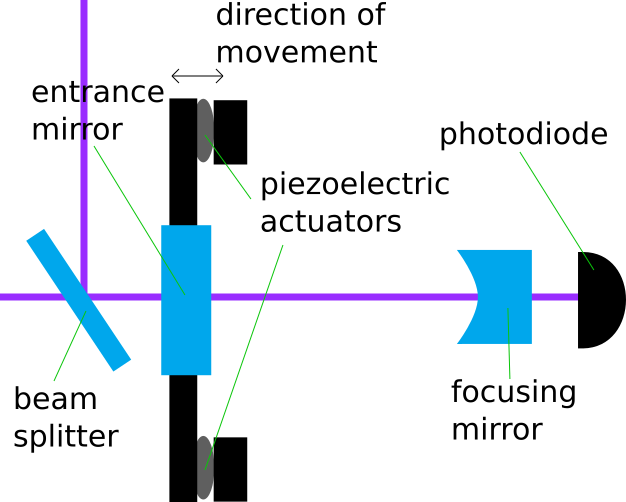
\includegraphics[trim=100pt 100pt 100pt 100pt, clip=true, totalheight=0.5\textheight,angle=90]{spectrumAnalyzer}}
    \centerline{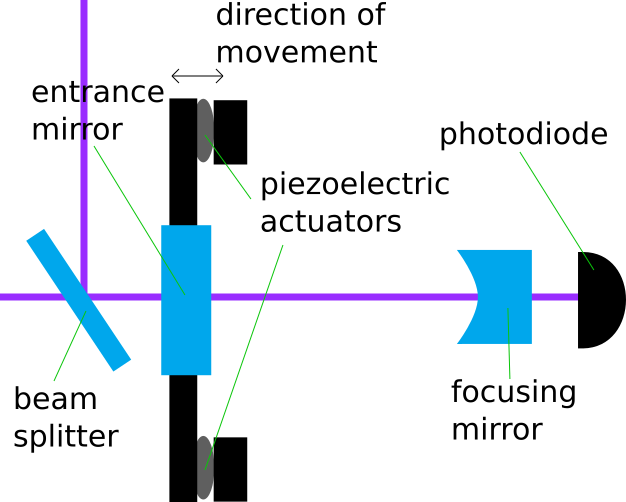
\includegraphics[totalheight=0.3\textheight ]{spectrumAnalyzer}}
    %\includegraphics[totalheight=0.3\textheight]{testfigure}
    \caption[]{\label{fig:spectrumAnalyzer}
    A diagram of the spectrum analyzer. both lasers are coupled to the cavity. One of the mirrors is mounted on piezoelectric devices that allow fine control of its motion. 
}
\end{figure} 

The spectrum analyzer is a semiconfocal cavity of length 200 mm. The flat, partially reflective mirror through which light enters the cavity is mounted on a mount that features piezo-electric actuators. At the other end is a curved mirror of focal length 200 mm. Behind this is a photodiode \footnote{the Thorlabs DET XXXXX--probably a DET100A/M or something similar.}.
The length of the optical cavity in the spectrum analyzer is thus modulated by sweeping the voltage that we put across the piezoelectric crystals. When the cavity length is such that the coupled light is close to a resonance of the cavity, we expect to see higher signal on the photodiode. 
The piezoelectric actuators are connected to a commercially available piezo control box that sweeps the voltage in a sawtooth wave type pattern, with a frequency $\sim$20Hz. 

The free spectral range of the spectrum analyzer describes exactly how far apart we expect the peaks to be. In the case of a hemiconfocal cavity like ours, the free spectral range is given by 

\begin{equation}
    \textnormal{FSR}=\frac{c}{8L}
\end{equation}
